\section{The Vehicle}

\subsection{The vehicle in general?}

\subsection{Gear ratio}


 \begin{figure}[H]
	\centering
	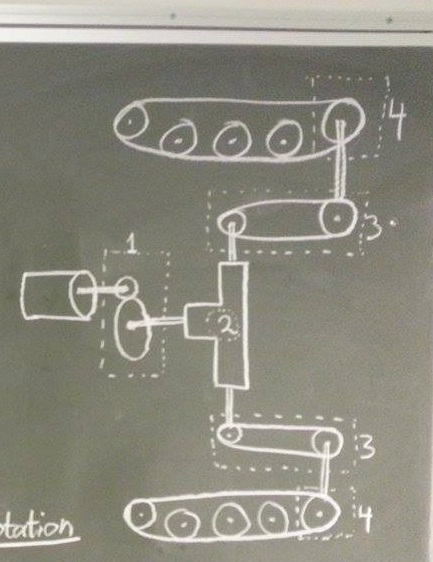
\includegraphics[scale=0.8]{figures/Drivetrain.jpg}
	\caption{Displays a sketch of the vehicles drivetrain}
	\label{fig:Drivetrain}
\end{figure}

\subsection{Needed power}

\subsection{Hall Sensor}

On the vehicle there are implemented two hall sensors, one on each belt. A hall sensor is a sensor that is activated, when it is exposed to a magnetic field. The sensors are placed beside the wheel \todo{Thomas: Or gear, what do we call it??}, on which there is two magnets. The magnets is placed, so that there is a half turn between them. The hall sensor is illustrated on figur \figref{HallSensor}.

 \begin{figure}[H]
	\centering
	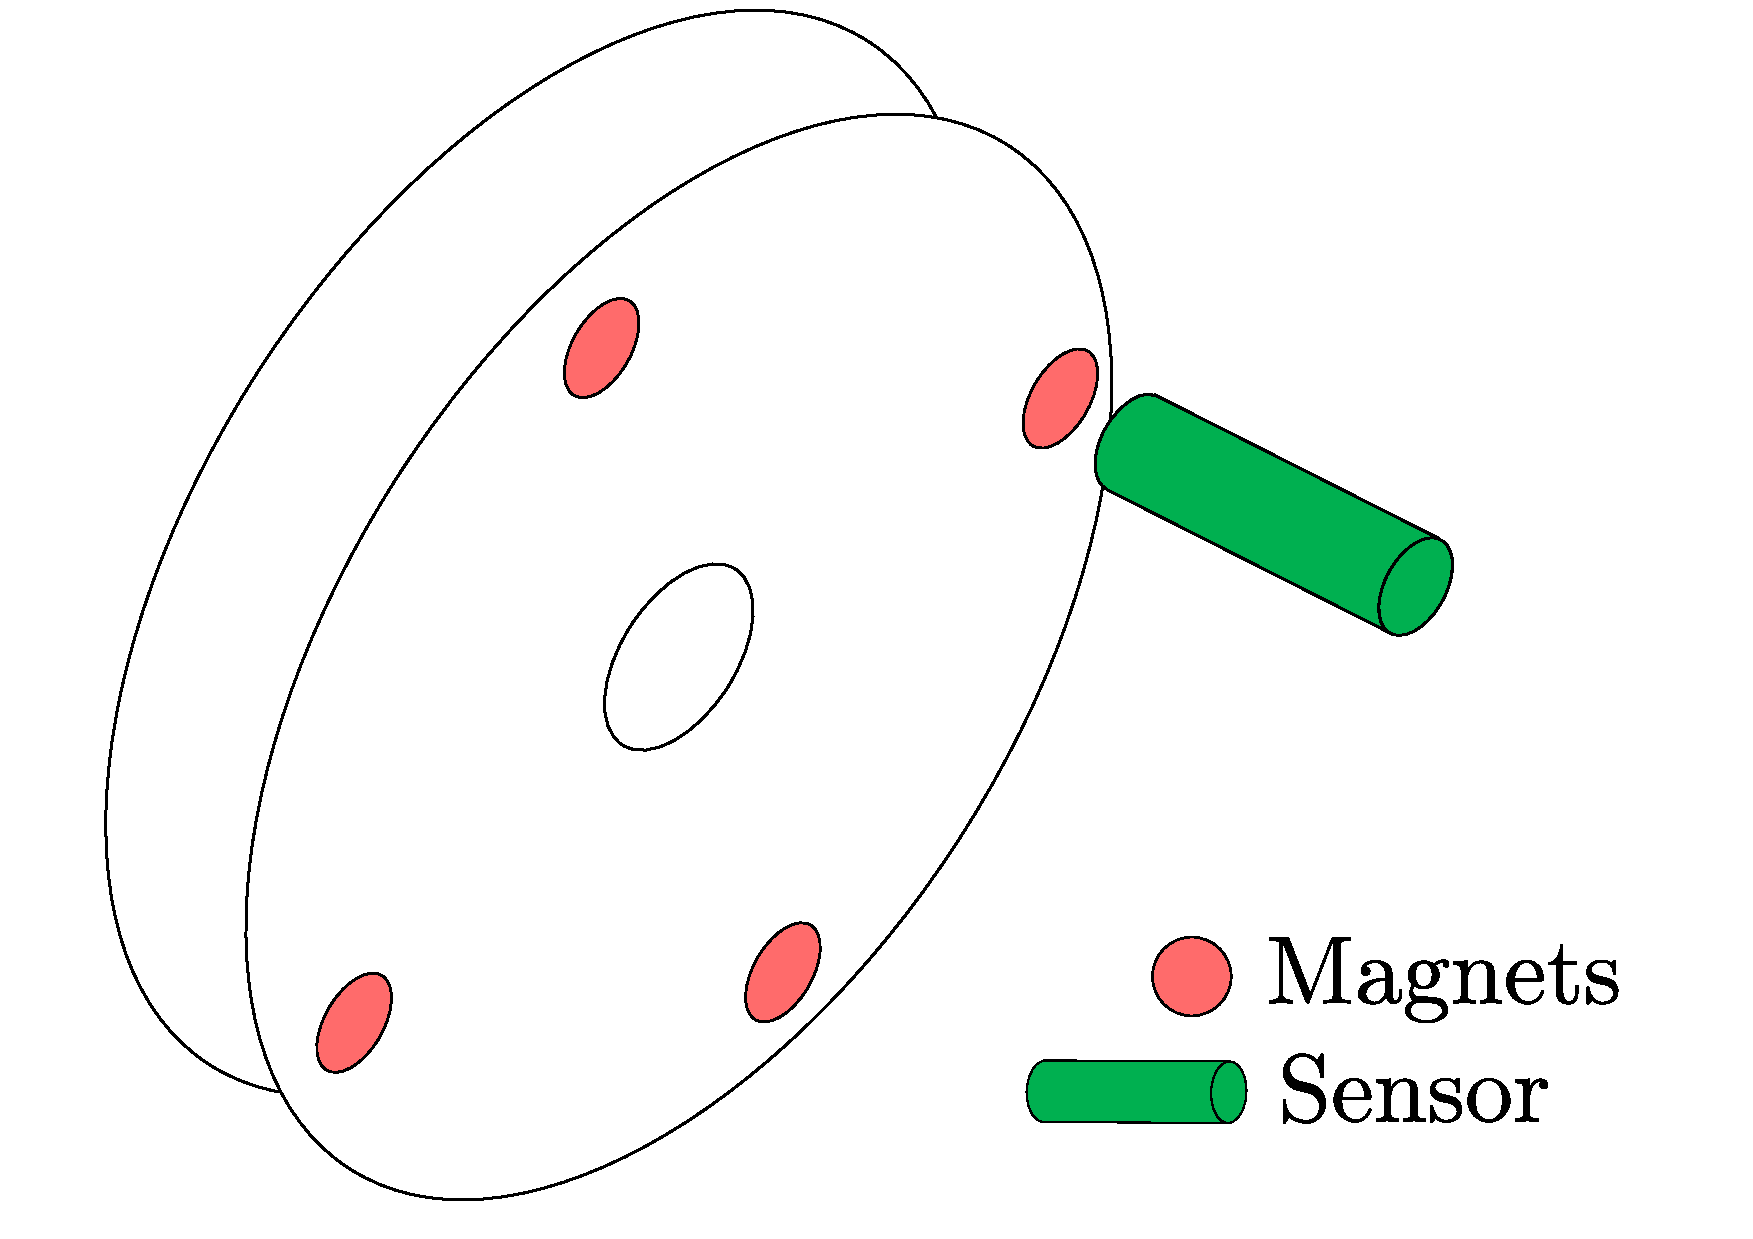
\includegraphics[scale=0.5]{figures/HallSensorSide_Forward_view.pdf}
	\caption{Illustration of the hall sensor, side view to the left and front view to the right. The red circles are the magnets and the green rectangle is the hall sensor.}
	\label{fig:HallSensor}
\end{figure}

The Hall sensor will give a voltage output, each time one of the magnets is in front of the hall sensor. This will give a output each half turn of the wheel. By knowing the time, a half turn will takes, by measurer the time between two outputs, and the distance, that the vehicle travel on a half a turn of the wheel, the speed of the vehicle can be calculated.
When the vehicle is starting the move, the first output from the hall sensor can not be used. This is because there will not be a output from the last pass by of a magnet and here of, the time for a half turn is not know. Therefore can the speed not be calculated by the first output, but first after the second output.

